\hypertarget{bbssp_8c}{
\section{/Users/johnlarusic/Dev/arrow2/src/bin/bbssp.c File Reference}
\label{bbssp_8c}\index{/Users/johnlarusic/Dev/arrow2/src/bin/bbssp.c@{/Users/johnlarusic/Dev/arrow2/src/bin/bbssp.c}}
}
Bottleneck Biconnected Spanning Subgraph solver. 

{\tt \#include \char`\"{}arrow.h\char`\"{}}\par
{\tt \#include $<$getopt.h$>$}\par


Include dependency graph for bbssp.c:\nopagebreak
\begin{figure}[H]
\begin{center}
\leavevmode
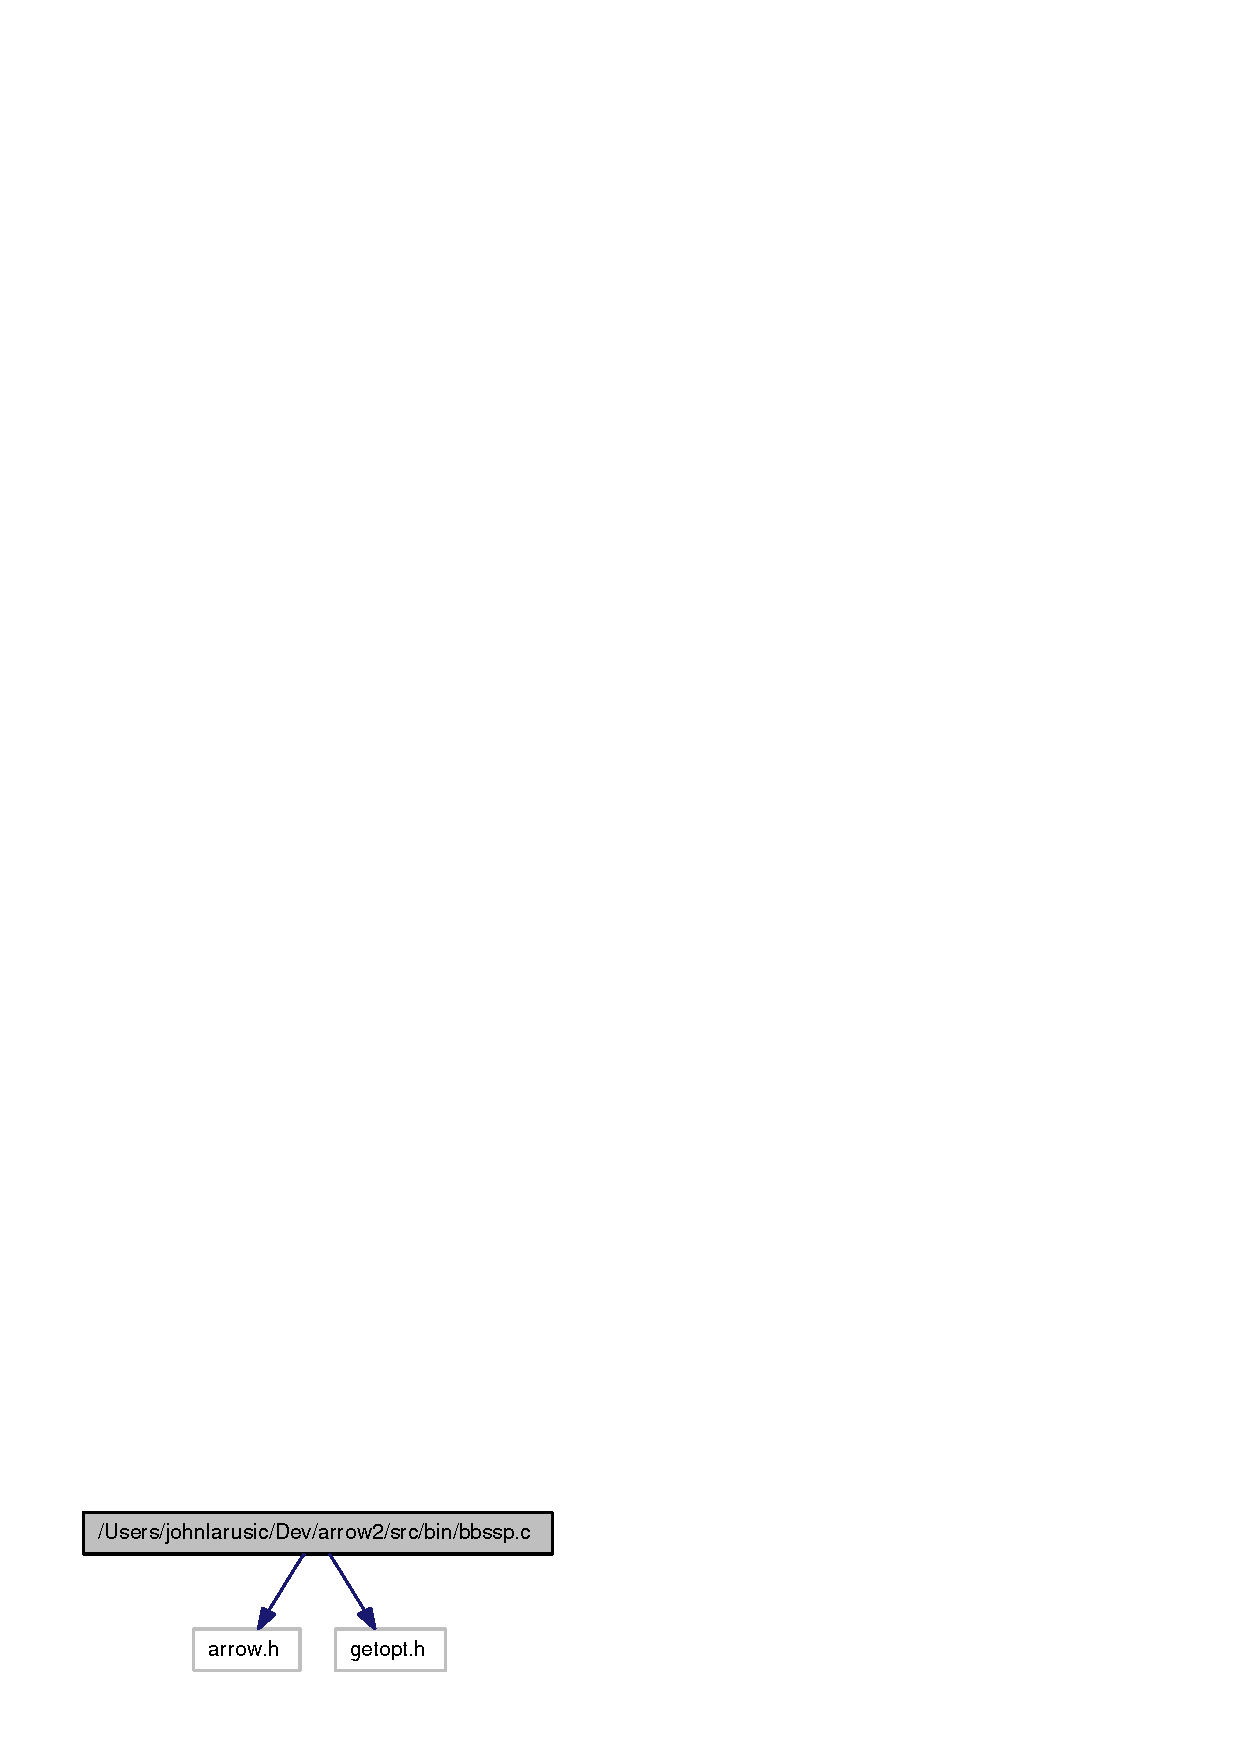
\includegraphics[width=134pt]{bbssp_8c__incl}
\end{center}
\end{figure}
\subsection*{Functions}
\begin{CompactItemize}
\item 
int \hyperlink{bbssp_8c_0ddf1224851353fc92bfbff6f499fa97}{main} (int argc, char $\ast$argv\mbox{[}$\,$\mbox{]})
\begin{CompactList}\small\item\em Entry point to program. \item\end{CompactList}\item 
void \hyperlink{bbssp_8c_b090c3311cfe36c9908201e66e09a06b}{print\_\-help} (char $\ast$program\_\-name)
\begin{CompactList}\small\item\em Prints usage/help message. \item\end{CompactList}\item 
void \hyperlink{bbssp_8c_0e9eb03b516f80fc4b993ef37b334376}{print\_\-version} (char $\ast$program\_\-name)
\begin{CompactList}\small\item\em Prints version message. \item\end{CompactList}\item 
void \hyperlink{bbssp_8c_767128a69bdfad046920286832102a40}{print\_\-usage} (char $\ast$program\_\-name)
\begin{CompactList}\small\item\em Prints usage message. \item\end{CompactList}\end{CompactItemize}
\subsection*{Variables}
\begin{CompactItemize}
\item 
static char $\ast$ \hyperlink{bbssp_8c_12c5840a4d4cb5474b40008b577d36c4}{short\_\-options} = \char`\"{}hV\char`\"{}
\begin{CompactList}\small\item\em Short argument options to getopt. \item\end{CompactList}\item 
static struct option \hyperlink{bbssp_8c_b5b68aa8f898c499ca2c3092ecd9e552}{long\_\-options} \mbox{[}$\,$\mbox{]}
\begin{CompactList}\small\item\em Long argument options to getopt. \item\end{CompactList}\end{CompactItemize}


\subsection{Detailed Description}
Bottleneck Biconnected Spanning Subgraph solver. 

Solves the bottleneck biconnected spanning subgraph problem (BBSSP) problem on the given input files.

\begin{Desc}
\item[Author:]John LaRusic \end{Desc}


Definition in file \hyperlink{bbssp_8c-source}{bbssp.c}.

\subsection{Function Documentation}
\hypertarget{bbssp_8c_0ddf1224851353fc92bfbff6f499fa97}{
\index{bbssp.c@{bbssp.c}!main@{main}}
\index{main@{main}!bbssp.c@{bbssp.c}}
\subsubsection{\setlength{\rightskip}{0pt plus 5cm}int main (int {\em argc}, \/  char $\ast$ {\em argv}\mbox{[}$\,$\mbox{]})}}
\label{bbssp_8c_0ddf1224851353fc92bfbff6f499fa97}


Entry point to program. 



Definition at line 55 of file bbssp.c.

References long\_\-options, print\_\-help(), print\_\-usage(), print\_\-version(), and short\_\-options.\hypertarget{bbssp_8c_b090c3311cfe36c9908201e66e09a06b}{
\index{bbssp.c@{bbssp.c}!print\_\-help@{print\_\-help}}
\index{print\_\-help@{print\_\-help}!bbssp.c@{bbssp.c}}
\subsubsection{\setlength{\rightskip}{0pt plus 5cm}void print\_\-help (char $\ast$ {\em program\_\-name})}}
\label{bbssp_8c_b090c3311cfe36c9908201e66e09a06b}


Prints usage/help message. 

\begin{Desc}
\item[Parameters:]
\begin{description}
\item[{\em program\_\-name}]\mbox{[}in\mbox{]} name of program \end{description}
\end{Desc}


Definition at line 98 of file bbssp.c.

References print\_\-usage().

Referenced by main().\hypertarget{bbssp_8c_767128a69bdfad046920286832102a40}{
\index{bbssp.c@{bbssp.c}!print\_\-usage@{print\_\-usage}}
\index{print\_\-usage@{print\_\-usage}!bbssp.c@{bbssp.c}}
\subsubsection{\setlength{\rightskip}{0pt plus 5cm}void print\_\-usage (char $\ast$ {\em program\_\-name})}}
\label{bbssp_8c_767128a69bdfad046920286832102a40}


Prints usage message. 

\begin{Desc}
\item[Parameters:]
\begin{description}
\item[{\em program\_\-name}]\mbox{[}in\mbox{]} name of program \end{description}
\end{Desc}


Definition at line 126 of file bbssp.c.

Referenced by main(), and print\_\-help().\hypertarget{bbssp_8c_0e9eb03b516f80fc4b993ef37b334376}{
\index{bbssp.c@{bbssp.c}!print\_\-version@{print\_\-version}}
\index{print\_\-version@{print\_\-version}!bbssp.c@{bbssp.c}}
\subsubsection{\setlength{\rightskip}{0pt plus 5cm}void print\_\-version (char $\ast$ {\em program\_\-name})}}
\label{bbssp_8c_0e9eb03b516f80fc4b993ef37b334376}


Prints version message. 

\begin{Desc}
\item[Parameters:]
\begin{description}
\item[{\em program\_\-name}]\mbox{[}in\mbox{]} name of program \end{description}
\end{Desc}


Definition at line 112 of file bbssp.c.

Referenced by main().

\subsection{Variable Documentation}
\hypertarget{bbssp_8c_b5b68aa8f898c499ca2c3092ecd9e552}{
\index{bbssp.c@{bbssp.c}!long\_\-options@{long\_\-options}}
\index{long\_\-options@{long\_\-options}!bbssp.c@{bbssp.c}}
\subsubsection{\setlength{\rightskip}{0pt plus 5cm}struct option {\bf long\_\-options}\mbox{[}$\,$\mbox{]}\hspace{0.3cm}{\tt  \mbox{[}static\mbox{]}}}}
\label{bbssp_8c_b5b68aa8f898c499ca2c3092ecd9e552}


\textbf{Initial value:}

\begin{Code}\begin{verbatim}
{
        {"help", no_argument, 0, 'h'},
        {"version", no_argument, 0, 'V'}
}
\end{verbatim}
\end{Code}
Long argument options to getopt. 



Definition at line 44 of file bbssp.c.

Referenced by main().\hypertarget{bbssp_8c_12c5840a4d4cb5474b40008b577d36c4}{
\index{bbssp.c@{bbssp.c}!short\_\-options@{short\_\-options}}
\index{short\_\-options@{short\_\-options}!bbssp.c@{bbssp.c}}
\subsubsection{\setlength{\rightskip}{0pt plus 5cm}char$\ast$ {\bf short\_\-options} = \char`\"{}hV\char`\"{}\hspace{0.3cm}{\tt  \mbox{[}static\mbox{]}}}}
\label{bbssp_8c_12c5840a4d4cb5474b40008b577d36c4}


Short argument options to getopt. 



Definition at line 39 of file bbssp.c.

Referenced by main().